\documentclass[sigconf,anonymous,review]{acmart}

\setcopyright{none}
\settopmatter{printacmref=false}
\renewcommand\footnotetextcopyrightpermission[1]{}
\pagestyle{plain}
\acmConference[CS510 Project]{CS510 Course Project}{May 2026}{Urbana, IL, USA}
\acmYear{2026}
\copyrightyear{2026}

\usepackage{amsmath}
\usepackage{booktabs}
\usepackage{array}
\usepackage{tikz}
\usetikzlibrary{shapes.geometric}
\microtypesetup{expansion=false}
\setlength{\emergencystretch}{2em}

\newcommand{\zbase}{z_0}
\newcommand{\zout}{z}
\newcommand{\drel}{\delta_{\mathrm{rel}}}
\newcommand{\loss}{\mathcal{L}}
\newcommand{\lintervene}{\mathcal{L}_{\mathrm{rel}}}
\newcommand{\lanchor}{\mathcal{L}_{\mathrm{anchor}}}
\newcommand{\ldelta}{\mathcal{L}_{\Delta}}
\newcommand{\simfn}{\mathrm{sim}}
\newcommand{\RRB}{\mathrm{RRB}}


\title{Anchored Relational Residual Adaptation for CLIP}

\author{Anonymous Authors}
\affiliation{%
  \institution{Anonymous Institution}
  \country{}
}
\email{}

\begin{abstract}
CLIP-style dual encoders support open-vocabulary retrieval and zero-shot recognition, but they often score captions by object co-occurrence while underweighting relation, role, and binding edits. We study whether relation sensitivity can be added without replacing the pretrained embedding path. Relational Residual Bottlenecking (RRB) freezes OpenCLIP ViT-B/16 and learns a bounded, parser-free residual correction, $\zout=\mathrm{normalize}(\zbase+\alpha\drel)$, from multi-channel token bottlenecks on each branch. On staged ARO/SugarCrepe relation suites, the selected no-targeted strong-anchor checkpoint improves relation accuracy from the plain-adapter baseline's $0.6956$ to $0.7734$ while retaining COCO image-to-text R@1 of $0.7340$ and ImageNet top-1 of $0.6342$. Hard token bottlenecks and no-channel residual controls achieve relation gains only with much larger retrieval and zero-shot degradation. The experiments also give a useful negative result: structured relational counterfactuals matter, while the earlier targeted slot loss is not necessary. The claim is deliberately bounded. COCO retention remains seed-fragile, Winoground transfer is flat-to-negative, Flickr30k shows an image-to-text retrieval tax, and responsibility probes do not support semantic slot specialization.

\end{abstract}

\begin{CCSXML}
<ccs2012>
 <concept>
  <concept_id>10010147.10010257.10010258.10010259</concept_id>
  <concept_desc>Computing methodologies~Computer vision</concept_desc>
  <concept_significance>500</concept_significance>
 </concept>
 <concept>
  <concept_id>10002951.10003260.10003277</concept_id>
  <concept_desc>Information systems~Multimedia and multimodal retrieval</concept_desc>
  <concept_significance>300</concept_significance>
 </concept>
</ccs2012>
\end{CCSXML}

\ccsdesc[500]{Computing methodologies~Computer vision}
\ccsdesc[300]{Information systems~Multimedia and multimodal retrieval}

\keywords{vision-language models, CLIP, compositionality, residual adaptation, retrieval}

\begin{document}
\maketitle

\section{Introduction}

Contrastive image-text encoders such as CLIP have become default infrastructure for retrieval, zero-shot classification, and as frozen components inside larger multimodal systems~\cite{radford2021clip,ilharco2021openclip}. Their strength is broad alignment: a single embedding space makes many downstream comparisons cheap. The same coarse alignment can be a weakness for relational edits. Captions that preserve object vocabulary but swap roles, attributes, spatial relations, or word order may remain close in embedding space even when the correct image-text match should change~\cite{yuksekgonul2022bags,hsieh2023sugarcrepe,thrush2022winoground}.

This paper asks a narrow question: can a frozen CLIP encoder be made more sensitive to relational counterfactuals while keeping the pretrained embedding path dominant? We use ``guardrail'' only in this narrow technical sense: retention of retrieval and zero-shot behavior on held-out COCO and ImageNet checks. It does not refer to content safety, red-teaming, or policy filtering. Because the COCO check uses a 1,000-image subset, it serves as a signal for catastrophic retrieval collapse rather than a certificate of full retrieval parity.

The word ``dominant'' is central to the design. If a method obtains relation sensitivity by replacing the frozen embedding with a new representation, then a high relation score may only show that the adaptation has learned the staged benchmark. It does not show that the model still behaves like a useful CLIP encoder. In this project, the intended intervention is smaller: keep the original OpenCLIP representation available to every downstream dot product, and ask whether a relation-trained correction can move difficult counterfactual pairs just enough to change their ranking. This makes the evaluation asymmetric. A relation gain is necessary, but it is not sufficient. The gain must be read together with retrieval, zero-shot, residual-size, and external-validity checks.

This emphasis also determines how we interpret negative results. A hard bottleneck that improves relation accuracy but breaks COCO retrieval is not a partial success for the paper's claim; it is evidence that the relation signal is easy to overfit and difficult to add safely. A low residual norm is not automatically safe either, because two residuals with similar norm can point in different directions in embedding space and have different retrieval effects. The paper therefore treats each run as a point in a relation-preservation tradeoff rather than as a single scalar score.

The difficulty is visible in the project's early variants. Hard token bottlenecks can expose relation signal, but replacing the pretrained path damages broad CLIP behavior. A representative hard-token targeted run reaches relation accuracy $0.7488$, yet falls to COCO image-to-text R@1 $0.3920$ and ImageNet top-1 $0.0660$. In contrast, the selected RRB checkpoint reaches relation accuracy $0.7734$ with COCO R@1 $0.7340$ and ImageNet top-1 $0.6342$. The result is not lossless preservation, but it is a qualitatively different tradeoff.

The same caution applies to mechanism language. The implementation uses multiple latent residual channels, but the responsibility probes later in the project do not justify a claim that those channels become human-interpretable relation slots. We therefore use the channels as an architectural bottleneck: they constrain how the residual is computed from frozen token features, but the paper does not ask readers to believe that channel one means spatial relations or channel two means attributes. This distinction matters because the no-channel controls are relation-strong yet unsafe, while the responsibility probes are diffuse. The supported conclusion is about the residual interface and its guardrail behavior, not about discovered symbolic structure.

The paper is therefore a bottleneck-first study rather than a claim about rank-efficient adaptation in general. LoRA-style methods constrain parameter updates through rank, while RRB constrains the route from frozen token features to the final embedding correction. This difference is the object of study: we evaluate whether a narrow residual interface can carry relation supervision without letting the adapted path dominate the pretrained embedding.

We make four contributions.
\begin{enumerate}
    \item We define Relational Residual Bottlenecking (RRB), a parser-free residual adaptation module for frozen OpenCLIP image and text encoders.
    \item We show that RRB improves staged relation accuracy while avoiding the catastrophic retrieval and zero-shot collapse of hard bottlenecks and no-channel residual controls.
    \item We isolate the useful training signal: structured relational counterfactuals under residual anchoring, not generic hard negatives and not the earlier targeted relational loss.
    \item We report the limits directly: COCO retention is seed-fragile, Winoground is not improved, Flickr30k image-to-text retrieval drops, and responsibility probes do not justify semantic slot claims.
\end{enumerate}

\begin{figure*}[t]
    \centering
    % Auto-generated by figures/generate_paper_assets.py
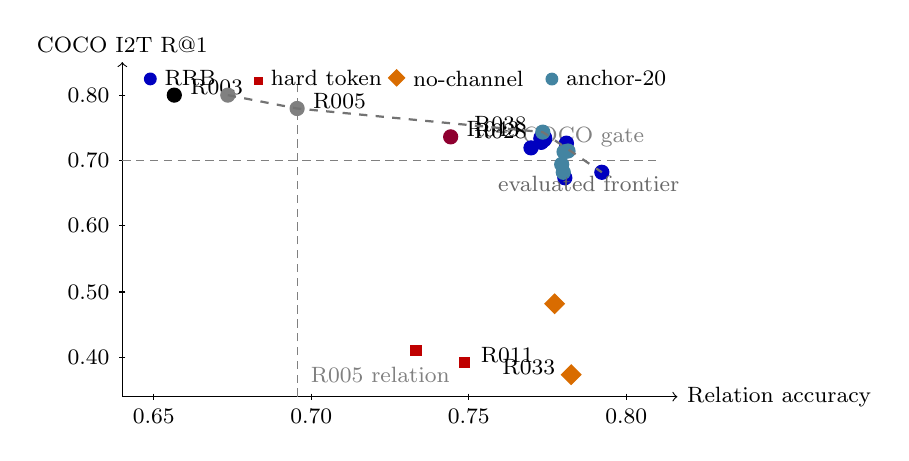
\begin{tikzpicture}[font=\footnotesize]
\draw[->] (0,0) -- (7.05,0) node[right] {Relation accuracy};
\draw[->] (0,0) -- (0,4.25) node[above] {COCO I2T R@1};
\draw (0.40,0.04) -- (0.40,-0.04) node[below] {0.65};
\draw (2.40,0.04) -- (2.40,-0.04) node[below] {0.70};
\draw (4.40,0.04) -- (4.40,-0.04) node[below] {0.75};
\draw (6.40,0.04) -- (6.40,-0.04) node[below] {0.80};
\draw (0.04,0.50) -- (-0.04,0.50) node[left] {0.40};
\draw (0.04,1.33) -- (-0.04,1.33) node[left] {0.50};
\draw (0.04,2.17) -- (-0.04,2.17) node[left] {0.60};
\draw (0.04,3.00) -- (-0.04,3.00) node[left] {0.70};
\draw (0.04,3.83) -- (-0.04,3.83) node[left] {0.80};
\draw[densely dashed,gray] (2.22,0) -- (2.22,4.00);
\draw[densely dashed,gray] (0,3.00) -- (6.80,3.00);
\node[gray,anchor=south west] at (2.27,0.05) {R005 relation};
\node[gray,anchor=south east] at (6.75,3.05) {COCO gate};
\node[circle,draw=black,fill=black,inner sep=1.8pt] (R003) at (0.66,3.83) {};
\node[anchor=west] at (0.74,3.93) {R003};
\node[circle,draw=gray,fill=gray,inner sep=1.8pt] (R005) at (2.22,3.66) {};
\node[anchor=west] at (2.30,3.76) {R005};
\node[rectangle,draw=red!75!black,fill=red!75!black,inner sep=1.8pt] (R011) at (4.35,0.43) {};
\node[anchor=west] at (4.43,0.53) {R011};
\node[rectangle,draw=red!75!black,fill=red!75!black,inner sep=1.8pt] (R014) at (3.73,0.59) {};
\node[circle,draw=blue!75!black,fill=blue!75!black,inner sep=1.8pt] (R019) at (5.19,3.16) {};
\node[circle,draw=blue!75!black,fill=blue!75!black,inner sep=1.8pt] (R023) at (6.09,2.85) {};
\node[circle,draw=gray,fill=gray,inner sep=1.8pt] (R024) at (1.34,3.83) {};
\node[circle,draw=blue!75!black,fill=blue!75!black,inner sep=2.3pt] (R028) at (5.34,3.28) {};
\node[anchor=east] at (5.26,3.38) {R028};
\node[circle,draw=blue!75!black,fill=blue!75!black,inner sep=1.8pt] (R029) at (5.32,3.23) {};
\node[circle,draw=blue!75!black,fill=blue!75!black,inner sep=1.8pt] (R031) at (5.64,3.22) {};
\node[circle,draw=blue!75!black,fill=blue!75!black,inner sep=1.8pt] (R032) at (5.62,2.78) {};
\node[diamond,draw=orange!85!black,fill=orange!85!black,inner sep=1.8pt] (R033) at (5.70,0.28) {};
\node[anchor=east] at (5.62,0.38) {R033};
\node[circle,draw=cyan!60!black,fill=cyan!60!black,inner sep=1.8pt] (R035) at (5.61,3.11) {};
\node[circle,draw=cyan!60!black,fill=cyan!60!black,inner sep=1.8pt] (R036) at (5.60,2.85) {};
\node[circle,draw=cyan!60!black,fill=cyan!60!black,inner sep=1.8pt] (R037) at (5.66,3.12) {};
\node[circle,draw=cyan!60!black,fill=cyan!60!black,inner sep=1.8pt] (R038) at (5.34,3.36) {};
\node[anchor=east] at (5.26,3.46) {R038};
\node[circle,draw=cyan!60!black,fill=cyan!60!black,inner sep=1.8pt] (R039) at (5.58,2.95) {};
\node[diamond,draw=orange!85!black,fill=orange!85!black,inner sep=1.8pt] (R040) at (5.49,1.18) {};
\node[circle,draw=purple!75!black,fill=purple!75!black,inner sep=1.8pt] (R043) at (4.17,3.30) {};
\node[anchor=west] at (4.25,3.40) {R043};
\draw[dashed,thick,black!55] (1.34,3.83) -- (2.22,3.66) -- (5.34,3.36) -- (6.09,2.85);
\node[black!60,anchor=west] at (4.65,2.70) {evaluated frontier};
\node[anchor=west] at (0.15,4.05) {\tikz\node[circle,draw=blue!75!black,fill=blue!75!black,inner sep=1.5pt]{}; RRB};
\node[anchor=west] at (1.55,4.05) {\tikz\node[rectangle,draw=red!75!black,fill=red!75!black,inner sep=1.4pt]{}; hard token};
\node[anchor=west] at (3.25,4.05) {\tikz\node[diamond,draw=orange!85!black,fill=orange!85!black,inner sep=1.5pt]{}; no-channel};
\node[anchor=west] at (5.25,4.05) {\tikz\node[circle,draw=cyan!60!black,fill=cyan!60!black,inner sep=1.5pt]{}; anchor-20};
\end{tikzpicture}

    \caption{Relation accuracy versus COCO image-to-text retrieval for key evaluated systems. Hard-token controls replace the pretrained embedding path with a bottlenecked representation, while no-channel controls use a residual path without the multi-channel bottleneck. The selected RRB checkpoint is shown as a point; seed dispersion for RRB variants is summarized separately in Figure~\ref{fig:seed_anchor}. Standard PEFT baselines such as LoRA and text-only tuning were not evaluated in this ablation study, which focuses on the architectural impact of the RRB bottleneck.}
    \Description{Scatter plot of relation accuracy against COCO image-to-text recall. OpenCLIP and the plain adapter sit at lower relation and high retrieval, hard-token and no-channel controls have higher relation but poor retrieval, and the selected RRB point sits between them with improved relation and bounded retrieval loss.}
    \label{fig:relation_coco}
\end{figure*}

This framing is intentionally conservative. The paper is not a claim that RRB solves compositional reasoning for CLIP. It is an empirical characterization of a useful relation-vs-preservation tradeoff and of the failure modes that remain.

The rest of the paper follows that framing. Section~2 positions RRB relative to compositional CLIP evaluation, structure-aware retrieval, and preservation-oriented adaptation. Section~3 defines the residual interface and training objective. Section~4 reports the run families and shows why the selected checkpoint is a tradeoff point rather than a universal improvement. Section~5 analyzes the remaining failures, including seed fragility, external retrieval degradation, and unsupported channel-interpretability claims.

\section{Related Work}

\paragraph{CLIP and compositional failures.}
CLIP learns transferable image representations from natural-language supervision and remains a common frozen backbone for retrieval and zero-shot transfer~\cite{radford2021clip,ilharco2021openclip}. Several benchmarks show that strong image-text encoders can still behave like bags of words or exploit benchmark artifacts rather than bind objects, attributes, and relations faithfully~\cite{yuksekgonul2022bags,hsieh2023sugarcrepe,thrush2022winoground}. Our experiments use ARO- and SugarCrepe-style relation suites as staged counterfactual checks, but we also include Winoground and Flickr30k follow-ups because benchmark-specific gains do not automatically imply broad compositional generalization.

The staged suites are useful because they create controlled caption alternatives: many words remain fixed while an order, object, attribute, or relation changes. That format makes the relation failure easy to measure with a dual encoder. It is also limited. A model can learn to separate benchmark-style edits without acquiring the full visual grounding needed for natural paired-image binding. Winoground was included for exactly this reason. It asks for paired discrimination across two images and two captions, which is closer to a binding test than a single counterfactual ranking margin. The negative Winoground result in Section~4 therefore narrows the paper's claim rather than contradicting it.

Recent benchmark and prompting studies point to the same caution from different directions. Multi-image relation tests, causal-order probes, and visual causal reasoning suites show that modern vision-language models can struggle when the correct answer depends on inter-image structure, event order, or counterfactual intervention rather than object presence alone~\cite{zong2024mirb,komanduri2025causalvlbench,weng2026causalorder}. Compositional chain-of-thought prompting can elicit more explicit decompositions from large multimodal models~\cite{mitra2024ccot}, but RRB targets the lower-level dual-encoder setting where inference remains a single dot product between independently encoded image and text embeddings.

\paragraph{Structured image-text matching.}
Graph and structure-aware image-text retrieval methods explicitly represent objects and relations, often through scene graphs, relationship-enhanced semantic graphs, triple-level relation reasoning, dynamic multi-relational graphs, or multi-level semantic matching~\cite{wang2019crossmodal,liu2024resg,ma2026tsgr2,liu2024semscene,song2025cmrgr,chen2024spatialvlm}. These methods motivate the relation failure mode, but they differ from RRB's constraint: inference remains a normal dual encoder with no detector, parser, cross-encoder, graph extractor, or reranker. RRB uses structured counterfactuals as training supervision while keeping the runtime embedding interface unchanged.

This distinction is practical as well as conceptual. A cross-encoder or graph matcher can inspect a candidate image-caption pair jointly, but a CLIP-style retrieval index usually relies on precomputed embeddings and dot products. Changing that interface changes storage, indexing, latency, and downstream compatibility. RRB deliberately avoids that route. The method can be viewed as asking how much relation sensitivity can be added while still exporting one image vector and one text vector. This constraint makes the method weaker than explicit reasoning systems in some settings, but it makes the preservation problem more precise.

A related line uses structured knowledge or explicit visual structure to improve multimodal reasoning and pretraining. Examples include 3D scene-graph guided pretraining, unified multimodal knowledge graph protocols, annotation-free multimodal knowledge-graph construction, graph-conditioned reasoning with large language models, and structural-cue enhanced CLIP training~\cite{liu20243dscenegraph,gong2024uknow,liu2025valik,sun2026mario,ruan2026structxlip}. These papers strengthen the motivation for relational structure, but most either introduce extra structured inputs, graph construction, or model-scale reasoning machinery. RRB is deliberately smaller: it asks whether relation supervision can be absorbed into a frozen OpenCLIP-style embedding interface without changing retrieval-time inputs.

There is also a more distant family of latent-interface work that transfers internal states directly, such as KV-cache alignment or cache-to-cache communication between language models~\cite{dery2026latentcache,fu2026cachetocache}. RRB is not a communication protocol and does not pass caches between models, but this nearby literature is useful context for treating internal representation interfaces as design objects rather than only as hidden implementation details.

\paragraph{Relation-aware CLIP adaptation.}
Recent relation-aware CLIP work, including RACA-CLIP-style alignment efforts, targets compositional relation sensitivity directly. The local RACA-CLIP manuscript available in this project is under-review with incomplete bibliographic metadata, so we treat it as conceptual prior art rather than assign unsupported venue metadata~\cite{raca2026local}. The distinction is that RRB focuses on preserving the frozen model's retrieval and zero-shot anchor through a bounded residual path. The novelty is not ``using relations'' alone; it is the residualized tradeoff analysis plus the evidence that hard replacement bottlenecks are unsafe for broad alignment.

That positioning is intentionally modest. Relation supervision, counterfactual captions, and CLIP adaptation are active areas, so the contribution cannot rest on the existence of relational data. The evidence in this project is instead diagnostic: the same broad recipe can yield very different guardrail behavior depending on whether the pretrained path is replaced, residualized, bottlenecked, or unconstrained. The hard-token runs establish that relation signal is reachable but unsafe under replacement. The generic-negative run establishes that ordinary hard-negative mining does not reproduce the relation gain. The no-channel controls establish that a residual path without the bottleneck can still damage retrieval badly. These comparisons are the reason the method section emphasizes architecture and objective together.

\paragraph{Preservation-oriented adaptation.}
Residual adapters, low-rank adaptation, and null-space or principal-subspace constraints are natural tools for changing a pretrained model while limiting drift~\cite{hu2022lora,peng2025gnsp,luo2026keeplora,qiao2024pegp,wu2026psoft,lu2024vptnullspace}. We do not claim that residual adaptation or orthogonal projection is novel. In fact, the ROP follow-up in this project is framed as a preservation ablation and future direction, not as the headline method. The supported contribution is more specific: structured relational counterfactual training through a bounded residual interface, together with guardrail diagnostics showing where this interface helps and where it fails.

The missing standard PEFT baselines are an important limitation. LoRA, text-only tuning, vision-only tuning, prompt tuning, and related low-rank or subspace methods could offer different relation-preservation tradeoffs. This draft does not claim that RRB dominates them. Its narrower question is bottleneck-versus-unconstrained residual routing, not rank-constrained adaptation. Within the implemented run family, the bounded multi-channel residual interface avoids the most severe failures observed in hard replacement and no-channel residual controls. A stronger submission would need to place RRB against common adaptation baselines directly.

\section{Relational Residual Bottlenecking}

\subsection{Setup}

Let $f_v$ and $f_t$ be frozen OpenCLIP image and text encoders. For an image $I$ or caption $T$, the frozen model produces normalized embeddings $\zbase^v=f_v(I)$ and $\zbase^t=f_t(T)$. The goal is to adjust the embedding used for contrastive comparison without discarding $\zbase$, since the pretrained path carries the broad retrieval and zero-shot behavior that we want to retain.

The method is designed for the dual-encoder setting. At inference time, images and captions must still be embeddable independently, and the final similarity remains a dot product between normalized vectors. No detector, parser, cross-attention reranker, scene graph, or candidate-pair module is added. This choice rules out some stronger reasoning machinery, but it keeps the evaluation focused on whether a pretrained embedding can be corrected rather than replaced.

RRB attaches a small trainable residual module to each branch:
\begin{equation}
    \zout^b = \mathrm{normalize}\left(\zbase^b + \alpha \drel^b\right), \qquad b \in \{v,t\}.
    \label{eq:rrb}
\end{equation}
Here $\drel^b$ is computed from CLIP token features through a parser-free multi-channel bottleneck and $\alpha$ is a fixed residual gate. The selected checkpoint uses $\alpha=0.05$. The residual therefore has to act as a correction to the original representation rather than a replacement representation.

The fixed gate is deliberately simple. A learned gate can increase flexibility, but the early R022 diagnostic run, omitted from the main tables for brevity, showed that more flexible residual control can still miss the COCO gate. A fixed gate is preferred because it maintains the architectural prior of a dominant pretrained path throughout training, preventing the residual branch from taking over the embedding space through an unconstrained mixing coefficient. The selected method fixes the residual scale and lets the objective decide when the residual direction is useful. This makes the resulting claims easier to audit: if guardrails fail, the failure cannot be attributed to an unbounded learned mixing coefficient silently replacing the frozen path.

\subsection{Multi-Channel Residual Interface}

For each branch, the module receives the frozen token sequence and induces $K$ latent channel states through learned queries and one self-attention block. The channel states are pooled and projected to the CLIP embedding dimension, producing $\drel^b$. We avoid the term ``semantic slots'' for the main method because later responsibility probes do not show semantic specialization. The bottleneck is used as an architectural constraint on the residual path, not as an interpretability claim.

The no-channel controls are important because they isolate this interface. R033 and R040 remove the multi-channel bottleneck and use a simpler residual adapter. Both remain relation-strong but damage retrieval and zero-shot behavior much more than RRB, suggesting that the bottlenecked residual interface is preservation-relevant even though its channels are not semantically interpretable.

The interface can be understood as a capacity and routing prior. The residual is not produced by one unconstrained multilayer projection from all token features to the final embedding. Instead, the token sequence must be summarized through a small number of channel states before it can affect the CLIP vector. This is not a guarantee of safety, and the seed results show that it is not enough by itself. It does, however, create a narrower path for the relation objective to act through. The contrast between R028 and the no-channel controls is consistent with this interpretation: similar or stronger relation accuracy can be achieved without the channel interface, but the resulting embedding drift is far more harmful to COCO and ImageNet.

This caution is consistent with recent analyses of ViT token aggregation, which show that global tokens can rely on background-dominated shortcut patches under coarse supervision~\cite{shi2026lastvit}. RRB does not attempt to fix dense-feature artifacts. The relevance is narrower: token summaries are not automatically benign, so the paper evaluates the final residual direction through retrieval and zero-shot guardrails instead of assuming that a small token-derived correction is safe.

The paper therefore separates three ideas that are easy to conflate. First, multiple channels are an architectural bottleneck. Second, the channels might become specialized in some future model. Third, the current probes do not show that specialization. Only the first statement is part of the method claim. The second is a hypothesis, and the third is a negative result reported in Section~4.

\subsection{Training Objective}

Training uses structured relation counterfactuals and anchor examples:
\begin{equation}
    \loss =
    \lambda_{\mathrm{rel}}\lintervene
    + \lambda_{\mathrm{anchor}}\lanchor
    + \lambda_{\Delta}\ldelta .
    \label{eq:loss}
\end{equation}
$\lintervene$ is a margin ranking loss over structured relation edits. Given a positive pair $(I,T^+)$ and a counterfactual caption $T^-$ that changes a relation, role, order, object, or attribute while preserving much of the surface vocabulary, the loss encourages $\simfn(\zout^v_I,\zout^t_{T^+})$ to exceed $\simfn(\zout^v_I,\zout^t_{T^-})$ by a margin. The same principle applies to branch-specific counterfactuals where available.

$\lanchor$ is feature mimicry on anchor pairs:
\begin{equation}
    \lanchor =
    \left\|\zout^v - \zbase^v\right\|_2^2 +
    \left\|\zout^t - \zbase^t\right\|_2^2 .
\end{equation}
It keeps the adapted embeddings close to the frozen OpenCLIP anchor on examples that should not require relational correction. $\ldelta$ penalizes residual magnitude,
\begin{equation}
    \ldelta = \left\|\drel^v\right\|_2^2 + \left\|\drel^t\right\|_2^2,
\end{equation}
which works with the fixed gate in Eq.~\ref{eq:rrb} to bound feature drift.

An earlier targeted relational loss attempted to localize edited spans to particular bottleneck channels. The final method removes that term. The ablations show that structured counterfactual supervision and residual anchoring are sufficient for the observed relation gain; the targeted loss is not necessary and should not be used as a mechanism claim.

\subsection{Structured Counterfactual Signal}

The relation loss depends on counterfactual captions whose surface form is close to the positive caption but whose relation, role, object, attribute, or order is changed. This structure is what distinguishes the method from generic hard-negative mining. Generic negatives can be visually or semantically difficult, but they need not isolate the binding error that CLIP tends to miss. In R024, generic hard negatives preserve broad OpenCLIP behavior almost perfectly, yet relation accuracy falls below the plain adapter baseline. That run is important because it rules out a simpler explanation: the selected model is not merely benefiting from more difficult negatives. It benefits from negatives that target the intended failure mode.

The training signal is also deliberately branch-compatible. Both image and text branches keep their frozen encoders, and both branches receive residual modules. The margin objective is evaluated through the final normalized embeddings, so the residual is rewarded only when it improves the contrastive comparison used by retrieval. This keeps the objective aligned with the deployed interface, although it also means that benchmark-specific counterfactual patterns can be learned without broader binding generalization. The Winoground and Flickr30k checks are included to expose that risk.

\subsection{Anchor Examples and Residual Regularization}

The anchor term uses examples that should not require a relational correction and asks the adapted embedding to mimic the frozen OpenCLIP embedding. This term is not a generic preference for small weights; it is a feature-space constraint at the point where downstream retrieval operates. The residual penalty is complementary. $\lanchor$ constrains the final normalized output on anchor examples, while $\ldelta$ constrains the branch residual itself. In the selected R028 configuration, $\lambda_{\mathrm{anchor}}=10$, $\lambda_{\Delta}=0.01$, and the anchor ratio is $0.75$.

The ablations show why both the anchor objective and the residual direction matter. R023 has low residual magnitude and high cosine to the frozen embedding, but it still misses the COCO gate. R028 keeps a similar small-residual regime and passes the pilot gate. R029 reintroduces the targeted loss and has a larger residual than R028 with no relation advantage. Anchor-20 runs reduce residual magnitude further but do not eliminate COCO seed fragility. The method should therefore be read as a bounded residual recipe, not as a theorem that smaller residuals are always safer.

\subsection{Model Selection Rule}

During experimentation, candidate checkpoints were evaluated with a pilot gate: relation accuracy had to exceed the plain adapter, COCO image-to-text R@1 had to be at least $0.70$, and ImageNet top-1 had to be at least $0.55$. This gate is not a universal deployment criterion. It is a project-level guard against selecting a model that wins the staged relation suite by destroying broad alignment. R028 is selected because it satisfies this gate while removing the unsupported targeted loss from the method. The seed studies then test how stable that selection is, rather than treating the selected checkpoint as sufficient evidence by itself.

For any practical use, this gate should be applied as a validation protocol rather than as a one-shot model choice. Multiple seeds should be trained under the same configuration; checkpoints that fail the relation, COCO, or ImageNet gates should be discarded; and the reported model should be accompanied by the seed pass rate. This protocol does not remove seed fragility, but it makes the fragility explicit and prevents relation-only selection from silently choosing an unsafe residual direction.

\section{Experiments}

\subsection{Setup}

All runs use OpenCLIP ViT-B/16 with LAION2B weights. The image and text encoders are frozen; only the adaptation modules are trainable. The selected R028 configuration uses $K=8$ residual channels, fixed residual gate $\alpha=0.05$, $\lambda_{\mathrm{anchor}}=10$, $\lambda_{\Delta}=0.01$, anchor ratio $0.75$, and no targeted relational loss. Remote jobs ran on RTX A6000 GPUs with no wandb logging.

The staged relation evaluation combines ARO/SugarCrepe-style relation and compositional counterfactual suites. Guardrail checks use COCO retrieval with 1,000 images and 5,002 captions, plus ImageNet zero-shot with 5,000 examples. External follow-ups use Winoground's 400 examples and Flickr30k retrieval with 1,000 images. The pilot gate used during experimentation required relation accuracy above the plain adapter, COCO image-to-text R@1 at least $0.70$, and ImageNet top-1 at least $0.55$.

The evaluation is organized by run families rather than isolated best checkpoints. R003 is frozen OpenCLIP. R005 is the plain adapter baseline. R011 and R014 are representative hard-token bottlenecks that replace the embedding path. R019, R025, and R027 are full RRB seed checks. R023, R028, R031, R032, and R035--R039 remove the targeted loss under different anchoring settings. R024 replaces structured relation counterfactuals with generic hard negatives. R033 and R040 remove the multi-channel bottleneck from the residual interface. R034, R041, R043, and R045 are follow-ups for external validity, mechanism, orthogonal projection, and Flickr30k retrieval.

The reported metrics are intentionally mixed. Relation accuracy measures the targeted failure mode, calculated as the simple average accuracy across all evaluated ARO and SugarCrepe sub-suites. COCO image-to-text R@1 measures whether the image embedding still retrieves the correct caption from a small held-out retrieval pool. ImageNet top-1 measures zero-shot category transfer. Residual magnitude and cosine-to-$\zbase$ summarize how much the adapted vector moves, but they are diagnostic rather than decisive. Winoground text, image, and group scores test a different binding setting, and Flickr30k checks whether the retrieval tradeoff transfers beyond the COCO guardrail split.

All numbers in this section come from the consolidated local experiment report and the copied remote-output summaries. The draft does not rerun the GPU training jobs during paper generation. That matters for interpretation: the paper is a faithful analysis of the existing run record, not a new benchmark campaign with exhaustive hyperparameter search.

% Auto-generated by figures/generate_paper_assets.py
\begin{table*}[t]
\centering
\caption{Main relation/anchor-preservation comparison. Relation accuracy is measured on staged ARO/SugarCrepe-style relation suites. COCO is image-to-text Recall@1 on the 1k-image guardrail split. Residual is the mean relative magnitude of the learned residual branch where available.}
\label{tab:main_results}
\small
\begin{tabular}{llrrrrrp{2.9cm}}
\toprule
Run & System & Relation & $\Delta$ vs R005 & COCO R@1 & ImageNet & Residual & Notes \\
\midrule
R003 & OpenCLIP & 0.6564 & -- & 0.7990 & 0.6670 & -- & Frozen OpenCLIP baseline \\
R005 & plain adapter & 0.6956 & 0.0000 & 0.7790 & 0.6438 & -- & Plain adapter baseline \\
R011 & hard token targeted & 0.7488 & 0.0532 & 0.3920 & 0.0660 & -- & Catastrophic guardrail degradation \\
R014 & hard token no targeted & 0.7332 & 0.0376 & 0.4110 & 0.0602 & -- & Catastrophic guardrail degradation \\
R019 & RRB full seed 1 & 0.7697 & 0.0741 & 0.7190 & 0.6152 & 0.1328 & Clears pilot guardrails \\
R028 & RRB no targeted, stronger anchor & 0.7734 & 0.0778 & 0.7340 & 0.6342 & 0.0804 & Selected configuration \\
R033 & no-slot residual adapter control & 0.7825 & 0.0869 & 0.3740 & 0.3308 & 0.2062 & Catastrophic guardrail degradation \\
R040 & constrained no-slot residual control & 0.7773 & 0.0817 & 0.4820 & 0.4798 & 0.0969 & Large retrieval/zero-shot degradation \\
\bottomrule
\end{tabular}
\end{table*}


\subsection{Main Tradeoff}

Table~\ref{tab:main_results} and Figure~\ref{fig:relation_coco} summarize the main tradeoff. In Figure~\ref{fig:relation_coco}, the selected configuration is highlighted with a star marker to distinguish it from other seed variations and baseline controls. OpenCLIP has the strongest broad guardrails among the core baselines, but lower relation accuracy. The plain adapter improves relation from $0.6564$ to $0.6956$ with a small guardrail tax. Hard token bottlenecks move relation further but collapse both guardrails: R011 reaches relation $0.7488$ with COCO R@1 $0.3920$ and ImageNet top-1 $0.0660$.

RRB demonstrates a distinct Pareto-style tradeoff compared with replacement bottlenecks. R019, the first full RRB seed, reaches relation $0.7697$ while passing the pilot COCO and ImageNet thresholds. The selected R028 checkpoint simplifies the method by removing the targeted loss and strengthening anchoring; it reaches relation $0.7734$, COCO R@1 $0.7340$, and ImageNet top-1 $0.6342$. This is still an alignment tax relative to OpenCLIP and the plain adapter, but it is not the catastrophic forgetting observed in the replacement bottlenecks.

The no-channel controls sharpen the interpretation. R033 reaches relation $0.7825$, higher than R028, but collapses COCO to $0.3740$ and ImageNet to $0.3308$. R040 constrains the same no-channel idea more strongly and reduces residual magnitude, but COCO remains only $0.4820$ and ImageNet $0.4798$. These controls show why relation accuracy cannot be optimized alone. They also support the architectural role of the multi-channel interface: a residual path without that bottleneck can find relation-improving directions that are incompatible with broad CLIP behavior.

The selected result is therefore a Pareto-style point, not a strict dominance claim. OpenCLIP and the plain adapter retain stronger retrieval. Some hard or unconstrained variants obtain relation scores close to or above R028. R028 is useful because it occupies a middle region that the earlier variants failed to reach: a substantial relation gain with retrieval and zero-shot scores still in a usable range. That is the paper's main empirical claim.

% Auto-generated by figures/generate_paper_assets.py
\begin{table}[t]
\centering
\caption{Structured counterfactuals, not the targeted relational loss $L_{targeted}$, explain the retained relation gain.}
\label{tab:ablation}
\small
\resizebox{\columnwidth}{!}{%
\begin{tabular}{llccrr}
\toprule
Run & Variant & Struct. CF & $L_{targeted}$ & Relation & COCO \\
\midrule
R023 & no-targeted, weak anchor & yes & 0 & 0.7922 & 0.6820 \\
R024 & generic hard negatives & no & 1 & 0.6736 & 0.7990 \\
R028 & selected stronger-anchor & yes & 0 & 0.7734 & 0.7340 \\
R029 & matched targeted control & yes & 1 & 0.7731 & 0.7280 \\
\bottomrule
\end{tabular}%
}
\end{table}


\subsection{What Training Signal Matters?}

Table~\ref{tab:ablation} separates structured counterfactual supervision from the targeted relational loss. R024 uses generic hard negatives rather than structured relational counterfactuals. It preserves COCO and ImageNet nearly perfectly, but relation accuracy drops to $0.6736$, below the plain adapter baseline. In contrast, R023 and R028 use structured counterfactuals with $L_{targeted}=0$ and retain large relation gains. R029 adds the targeted loss back under the same stronger-anchor setting and does not improve the selected tradeoff. The result is a useful anti-claim: the targeted loss sounded plausible but is not the supported mechanism.

This ablation is central because it prevents two overstatements. First, the gain is not explained by hard-negative training in general. If that were the explanation, R024 would have improved relation accuracy while preserving guardrails. It did the opposite: it preserved guardrails and lost the relation effect. Second, the gain is not evidence that targeted channel supervision discovers relation-specialized channels. R023 and R028 remove the targeted term entirely. R028 is the cleaner paper-facing method because it keeps the structured relation signal and the anchor terms while dropping a mechanism that the evidence does not need.

The R023/R028 comparison also shows why model selection cannot use relation accuracy alone. R023 reaches relation $0.7922$, higher than R028, but COCO falls to $0.6820$. R028 gives up some relation accuracy and passes the pilot guardrail. This tradeoff is exactly what the stronger anchor was meant to expose. The selected checkpoint is not the maximum relation model in the run history; it is the simplest relation-positive model that clears the explicit preservation gate.

% Auto-generated by figures/generate_paper_assets.py
\begin{table}[t]
\centering
\caption{Seed summaries for RRB variants. Values are mean $\pm$ sample standard deviation.}
\label{tab:seed_summary}
\small
\begin{tabular}{lrr}
\toprule
Group & Relation & COCO R@1 \\
\midrule
full RRB & 0.7768 $\pm$ 0.0062 & 0.6927 $\pm$ 0.0294 \\
anchor-10 no-targeted & 0.7782 $\pm$ 0.0042 & 0.7110 $\pm$ 0.0332 \\
anchor-20 no-targeted & 0.7789 $\pm$ 0.0032 & 0.7092 $\pm$ 0.0232 \\
\bottomrule
\end{tabular}
\end{table}


\subsection{Seed and Anchoring Stability}

\begin{figure}[t]
    \centering
    % Auto-generated by figures/generate_paper_assets.py
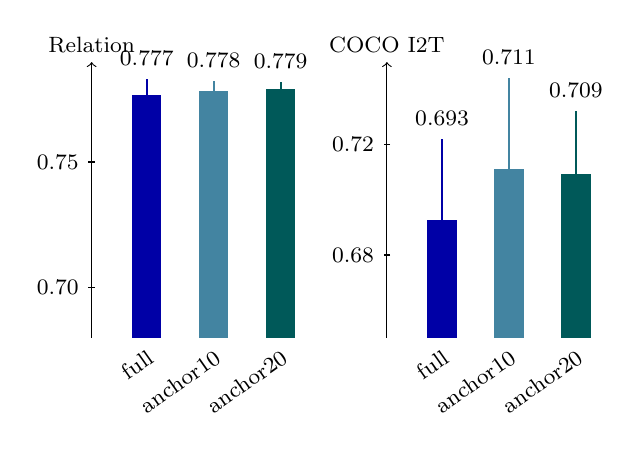
\begin{tikzpicture}[font=\footnotesize]
\draw[->] (0,0) -- (0,3.50) node[above] {Relation};
\draw[->] (3.75,0) -- (3.75,3.50) node[above] {COCO I2T};
\draw (0.04,0.64) -- (-0.04,0.64) node[left] {0.70};
\draw (0.04,2.23) -- (-0.04,2.23) node[left] {0.75};
\draw (3.79,1.05) -- (3.71,1.05) node[left] {0.68};
\draw (3.79,2.45) -- (3.71,2.45) node[left] {0.72};
\draw[fill=blue!65!black,draw=blue!65!black] (0.52,0) rectangle (0.88,3.08);
\draw[blue!65!black,thick] (0.70,2.88) -- (0.70,3.28);
\node[rotate=35,anchor=east] at (0.85,-0.15) {full};
\node[above] at (0.70,3.33) {0.777};
\draw[fill=blue!65!black,draw=blue!65!black] (4.27,0) rectangle (4.63,1.49);
\draw[blue!65!black,thick] (4.45,0.47) -- (4.45,2.52);
\node[rotate=35,anchor=east] at (4.60,-0.15) {full};
\node[above] at (4.45,2.57) {0.693};
\draw[fill=cyan!60!black,draw=cyan!60!black] (1.37,0) rectangle (1.73,3.13);
\draw[cyan!60!black,thick] (1.55,2.99) -- (1.55,3.26);
\node[rotate=35,anchor=east] at (1.70,-0.15) {anchor10};
\node[above] at (1.55,3.31) {0.778};
\draw[fill=cyan!60!black,draw=cyan!60!black] (5.12,0) rectangle (5.48,2.13);
\draw[cyan!60!black,thick] (5.30,0.97) -- (5.30,3.30);
\node[rotate=35,anchor=east] at (5.45,-0.15) {anchor10};
\node[above] at (5.30,3.35) {0.711};
\draw[fill=teal!70!black,draw=teal!70!black] (2.22,0) rectangle (2.58,3.15);
\draw[teal!70!black,thick] (2.40,3.05) -- (2.40,3.25);
\node[rotate=35,anchor=east] at (2.55,-0.15) {anchor20};
\node[above] at (2.40,3.30) {0.779};
\draw[fill=teal!70!black,draw=teal!70!black] (5.97,0) rectangle (6.33,2.07);
\draw[teal!70!black,thick] (6.15,1.26) -- (6.15,2.88);
\node[rotate=35,anchor=east] at (6.30,-0.15) {anchor20};
\node[above] at (6.15,2.93) {0.709};
\end{tikzpicture}

    \caption{Seed summaries show stable relation gains but imperfect COCO retention. Anchor-10 and anchor-20 no-targeted variants have similar mean COCO R@1 in these runs (0.711 and 0.709), so stronger anchoring does not eliminate retrieval performance degradation. Error bars are sample standard deviations.}
    \Description{Grouped summary chart comparing relation accuracy and COCO recall across full RRB, anchor-10 no-targeted RRB, and anchor-20 no-targeted RRB seed groups. Relation means are stable near 0.78, while COCO means vary and have nontrivial error bars.}
    \label{fig:seed_anchor}
\end{figure}

The seed summaries in Table~\ref{tab:seed_summary} and Figure~\ref{fig:seed_anchor} show stable relation gains and unstable retrieval retention. Full RRB over R019/R025/R027 has mean relation $0.7768 \pm 0.0062$, but mean COCO R@1 $0.6927 \pm 0.0294$, with only one of three runs clearing the COCO threshold. No-targeted anchor-10 runs R028/R031/R032 have mean relation $0.7782 \pm 0.0042$ and mean COCO $0.7110 \pm 0.0332$. Anchor-20 runs R035--R039 reduce residual drift in the consolidated diagnostics and keep relation stable, but their mean COCO remains $0.7092 \pm 0.0232$. The method therefore supports relation gains across seeds, not robust retrieval preservation across seeds.

The anchor-20 group is especially informative. It reduces mean residual magnitude to $0.0666$ and increases mean cosine-to-$\zbase$ to approximately $0.9975$, but this does not translate into a clearly higher COCO mean than the anchor-10 group. R038 is the best external-retrieval follow-up candidate in that group, yet other anchor-20 seeds still miss or nearly miss the COCO threshold. The result argues against a simple residual-size selection rule. Stronger anchoring can reduce drift, but relation-preserving directions and retrieval-preserving directions are not identical.

For a deployment-oriented paper, this would be a serious blocker. For this paper's more limited claim, it is part of the result. RRB gives a repeatable relation gain under multiple seeds and anchor settings, but retrieval preservation remains stochastic and incomplete. The right summary statistic is therefore not only the selected R028 point; it is the seed-group pass rate and variance around that point.

This is why the gate in Section~3.6 is a validation protocol rather than a guarantee. A relation-positive checkpoint is not considered usable until it also passes the COCO and ImageNet guardrails, and a run family is not considered stable unless its pass rate is reported. Under that stricter reading, R028 is evidence that a useful residual direction exists, while the seed table shows that the current training recipe does not find such directions reliably enough for deployment.

% Auto-generated by figures/generate_paper_assets.py
\begin{table*}[t]
\centering
\caption{External-validity and mechanism checks bound the claim. These follow-ups strengthen the limitation story rather than changing the main positive result.}
\label{tab:external_limits}
\small
\setlength{\tabcolsep}{3pt}
\begin{tabular}{p{2.1cm}p{4.1cm}p{7.7cm}}
\toprule
Check & Result & Interpretation \\
\midrule
\multicolumn{3}{l}{\textit{Downstream and external retrieval checks}} \\
Winoground R034 & R028 text/image/group 0.2400/0.1100/0.0700 vs OpenCLIP 0.2775/0.1075/0.0825 & Text and group scores drop while image score is nearly flat; no broad binding claim. \\
Flickr30k R045 & R028 I2T R@1 0.8260 vs OpenCLIP 0.8620; R038 0.8440 & External retrieval tax persists, smaller for anchor-20 R038. \\
\midrule
\multicolumn{3}{l}{\textit{Mechanistic and preservation probes}} \\
Slot responsibility R041 & entropy 1.0000, top-1 concentration 0.1259, edited overlap 0.1397 & Diffuse responsibility; no interpretable semantic-channel claim. \\
ROP ablation R043 & relation 0.7441, COCO 0.7360, ImageNet 0.6566 & Better preservation but relation gate fails; ROP remains an ablation/future direction. \\
\bottomrule
\end{tabular}
\end{table*}


\subsection{External Validity and Mechanism Checks}

Table~\ref{tab:external_limits} gives the boundary checks. Winoground does not support broad binding generalization: R028 scores $0.2400$ text, $0.1100$ image, and $0.0700$ group, while OpenCLIP scores $0.2775$, $0.1075$, and $0.0825$. Flickr30k confirms an external image-to-text retrieval tax: R028 drops from OpenCLIP's $0.8620$ to $0.8260$ I2T R@1, while R038 improves that to $0.8440$ but still does not match OpenCLIP. R041 responsibility probes are diffuse, with entropy near $1.0000$ and top-1 concentration near $0.126$, so the paper does not claim semantic channel specialization. R043's orthogonal-projection ablation preserves COCO and ImageNet better but fails the relation target, so it remains a cited ablation or future direction rather than a new headline.

The Winoground result is the cleanest warning against overgeneralization. R028 slightly improves image score by $0.0025$ over OpenCLIP but loses text and group score. A broad binding claim would require improvement on the group score, not only on staged ARO/SugarCrepe-style edits. The paper therefore treats Winoground as negative external-validity evidence. This is not surprising: the training signal emphasizes edited captions and margin ranking, while Winoground requires matching two captions and two images in a hand-curated setting where both visual and textual grounding must be correct.

Flickr30k gives a different warning. It is not a relation benchmark; it is an external retrieval distribution. The R028 image-to-text drop shows that the COCO guardrail is not a complete proxy for retrieval retention. R038 narrows the drop but does not close it. The text-to-image numbers are much closer to OpenCLIP, so an asymmetric retrieval tax is a plausible future-work hypothesis, not a claim established by the current small follow-up.

The responsibility probes close off the interpretability story. A useful semantic-channel result would show concentrated responsibility, consistent edited-token overlap, or stable channel assignments across examples. The observed entropy and top-1 concentration are close to diffuse. This does not invalidate the bottleneck as an architectural prior, but it does invalidate a stronger slot-semantics explanation. The final method name and captions therefore avoid promising interpretable slots.

\section{Analysis and Limitations}

\subsection{Residual Size Is Not Sufficient}

Residual magnitude is useful diagnostic information, but it is not a standalone safety predictor. R023 has low residual magnitude and high cosine to the frozen embedding, yet misses the COCO gate. R028 improves COCO under a similar small residual budget, while R029 has a larger residual and slightly lower COCO than R028. Anchor-20 runs reduce residual drift further, but do not solve COCO seed fragility. The direction and objective of the residual matter, not only its norm.

This point matters because residual methods are often described as safe by construction. RRB is safer than the hard replacement bottlenecks in this run history, but the residual form alone is not the safety argument. A residual can still move examples in directions that damage nearest-neighbor structure, which is also why preservation-oriented residual-gradient methods are relevant comparison points~\cite{luo2026keeplora}. Conversely, a moderately larger residual can be acceptable if it aligns with relation-sensitive distinctions while preserving the local neighborhoods that retrieval depends on. The experimental results suggest a more nuanced relationship: residual scale, anchor mimicry, and the multi-channel interface jointly improve the tradeoff, but none provides guaranteed preservation of all nearest-neighbor structures.

The selected checkpoint is best understood as a compromise between three pressures. The relation objective wants to separate edited captions that frozen CLIP tends to keep close. The anchor objective wants to keep clean examples near their frozen embeddings. The residual penalty wants the correction to stay small. When these pressures are balanced well, as in R028, relation accuracy improves with bounded degradation. When one pressure dominates or the interface is too unconstrained, the model either fails to learn relation sensitivity or damages retrieval.

\subsection{Generalization Gap}

The main positive result lives on staged relation/counterfactual suites. Those suites are useful because they isolate caption edits, but they are not equivalent to natural compositional reasoning. Winoground is hand-curated and requires paired text-image discrimination; R028 does not improve it. Flickr30k uses a different retrieval distribution and shows an external image-to-text tax. A plausible explanation is that structured counterfactual training teaches sensitivity to benchmark-style relational edits without fully learning the broader semantics needed for natural binding. This is a limitation, not a hidden success.

The per-source relation results reinforce this interpretation. R028 is strong on several SugarCrepe replacement categories and word-order checks, but ARO visual relation remains difficult, with left/right predicates dominating the failure taxonomy. This pattern suggests that the model is not simply acquiring a general spatial calculus. It learns useful distinctions for many edited captions, but some predicates remain close to the frozen model's blind spots. The improvement is therefore best described as counterfactual relation sensitivity, not full spatial reasoning.

The gap also affects how future data should be designed. Adding more edited captions of the same type may continue to improve the staged benchmark without improving Winoground or external retrieval. A stronger next experiment would include validation splits that are not generated by the same edit templates, paired-image binding checks, and retrieval datasets beyond COCO. The current paper uses external checks after the main run history to expose this issue; it does not claim to have solved it.

The objective itself explains part of the gap. Eq.~\ref{eq:loss} mostly contrasts one image with a positive caption and an edited caption. Winoground instead requires a two-image, two-caption decision where both cross-pair assignments must be correct. A natural next training signal is therefore image-pair contrast: construct paired images and paired captions that mimic the Winoground structure, then require the residual to improve the full assignment rather than only a single-image caption margin.

\subsection{Failure Taxonomy}

\begin{figure}[t]
    \centering
    \resizebox{\columnwidth}{!}{% Auto-generated by figures/generate_paper_assets.py
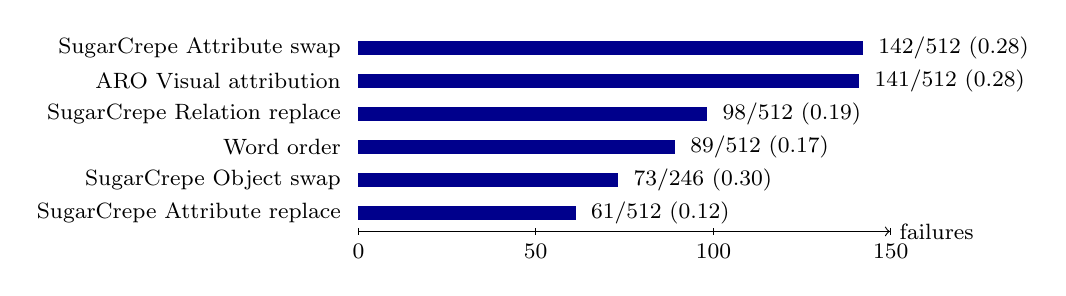
\begin{tikzpicture}[font=\footnotesize]
\node[anchor=east] at (-0.10,2.18) {SugarCrepe Attribute swap};
\draw[fill=blue!55!black,draw=blue!55!black] (0,2.10) rectangle (6.40,2.26);
\node[anchor=west] at (6.48,2.18) {142/512 (0.28)};
\node[anchor=east] at (-0.10,1.76) {ARO Visual attribution};
\draw[fill=blue!55!black,draw=blue!55!black] (0,1.68) rectangle (6.35,1.84);
\node[anchor=west] at (6.43,1.76) {141/512 (0.28)};
\node[anchor=east] at (-0.10,1.34) {SugarCrepe Relation replace};
\draw[fill=blue!55!black,draw=blue!55!black] (0,1.26) rectangle (4.42,1.42);
\node[anchor=west] at (4.50,1.34) {98/512 (0.19)};
\node[anchor=east] at (-0.10,0.92) {Word order};
\draw[fill=blue!55!black,draw=blue!55!black] (0,0.84) rectangle (4.01,1.00);
\node[anchor=west] at (4.09,0.92) {89/512 (0.17)};
\node[anchor=east] at (-0.10,0.50) {SugarCrepe Object swap};
\draw[fill=blue!55!black,draw=blue!55!black] (0,0.42) rectangle (3.29,0.58);
\node[anchor=west] at (3.37,0.50) {73/246 (0.30)};
\node[anchor=east] at (-0.10,0.08) {SugarCrepe Attribute replace};
\draw[fill=blue!55!black,draw=blue!55!black] (0,0.00) rectangle (2.75,0.16);
\node[anchor=west] at (2.83,0.08) {61/512 (0.12)};
\draw[->] (0,-0.15) -- (6.75,-0.15) node[right] {failures};
\draw (0.00,-0.11) -- (0.00,-0.19) node[below] {0};
\draw (2.25,-0.11) -- (2.25,-0.19) node[below] {50};
\draw (4.51,-0.11) -- (4.51,-0.19) node[below] {100};
\draw (6.76,-0.11) -- (6.76,-0.19) node[below] {150};
\end{tikzpicture}
}
    \caption{Largest remaining failure groups for the selected no-targeted, strong-anchor RRB model on the R030 diagnostic suite. The model still struggles with left/right spatial predicates, object and attribute swaps, and relation replacement cases.}
    \Description{Horizontal bar chart of remaining failure groups. The largest bars correspond to right-of and left-of spatial relations, followed by object swaps, attribute swaps, attribution, relation replacement, and word order.}
    \label{fig:failure_taxonomy}
\end{figure}

Figure~\ref{fig:failure_taxonomy} shows the largest remaining failure groups from the R030 diagnostic export for R028. Left/right spatial predicates remain difficult, and SugarCrepe object and attribute swaps still account for many errors. These failures are consistent with the external checks: RRB changes the relation-vs-preservation tradeoff, but it is not a complete spatial reasoning solution.

The margin information in the diagnostic report is also useful. The left/right failures have margins near zero, which means many examples are not confidently wrong by a large amount; they are ambiguous under the adapted similarity function. This is different from a failure where the model strongly prefers the counterfactual caption. Small margins suggest that additional supervision, better image grounding, or a more targeted residual direction constraint might move some examples. They do not by themselves show that the current model has the right abstraction.

Object and attribute swaps are a separate failure class. These are not purely spatial, and they indicate that the relation objective interacts with broader compositional binding. A method that only improves left/right predicates would not be enough. Conversely, a method that improves object and attribute swaps while losing retrieval may simply be changing the embedding geometry too broadly. The failure taxonomy therefore acts as a check on whether the residual is correcting the intended errors or merely shifting benchmark scores.

\subsection{Missing Baselines}

The available ablation suite compares RRB to OpenCLIP, a plain adapter, hard bottlenecks, generic hard negatives, no-targeted variants, no-channel residual controls, stronger anchoring, ROP, Winoground, and Flickr30k. It does not include standard PEFT baselines such as LoRA, text-only tuning, or vision-only tuning. While RRB shows stronger retention than naive residual controls in this study, its performance relative to widely used PEFT methods remains to be characterized in future work~\cite{hu2022lora}.

This missing-baseline caveat should change how the paper is read. The result is enough to support an internal method analysis: among the implemented designs, bounded multi-channel residual adaptation gives the best relation-preservation compromise. It is not enough to claim state-of-the-art adaptation. A direct PEFT comparison would need matched training data, the same guardrail metrics, seed repeats, and external retrieval checks. Without that, the paper should avoid language such as ``outperforms PEFT'' or ``dominates adapter baselines.''

The ROP follow-up is similarly bounded. Orthogonal or principal-subspace constraints are plausible preservation mechanisms, but they are close to existing null-space, gradient-projection, residual-gradient, and principal-subspace adaptation ideas~\cite{peng2025gnsp,luo2026keeplora,qiao2024pegp,wu2026psoft,lu2024vptnullspace}. R043 preserves COCO and ImageNet better than some RRB variants but fails the relation target. That makes it useful evidence about residual direction, not a replacement headline. The lack of relation gain in the ROP follow-up suggests that naive orthogonal constraints may be too restrictive for this training signal. We leave principal-subspace projection as a complementary guardrail to future work.

\subsection{Threats to Validity}

Several threats remain. First, the guardrail datasets are sampled. COCO uses a 1,000-image retrieval split and ImageNet uses 5,000 examples. These checks are large enough to catch catastrophic collapse, but they are not a full retrieval or zero-shot evaluation suite. Second, the relation suites are staged counterfactual benchmarks. They are valuable for isolating relation edits, but they may share template structure with the training signal. Third, the run history is a project campaign rather than a fully randomized hyperparameter study. Some comparisons are tightly matched, such as R028 versus R029, while others compare design families discovered over time.

Fourth, the paper evaluates embedding behavior, not downstream user tasks. Better relation sensitivity in a dual encoder may help retrieval, filtering, or ranking, but this draft does not test an end application. Fifth, the method is tied to OpenCLIP ViT-B/16 with LAION2B weights. Other backbones may have different baseline relation sensitivity and different tolerance for residual adaptation. Sixth, the external validity checks are negative or mixed. That makes the claim honest, but it also means that the method should not be presented as a broad compositional reasoning solution.

These threats do not erase the main result. They define its scope. The evidence supports a bounded statement about adding relation sensitivity through a residual interface while avoiding the worst guardrail failures in this run family. It does not support stronger claims about universal retrieval preservation, semantic channel discovery, or broad binding generalization.

\subsection{Practical Implications}

The practical lesson is to evaluate relation adaptation with guardrails from the beginning. If the project had selected only by relation accuracy, the hard bottlenecks and no-channel controls would have looked attractive. Their retrieval and zero-shot metrics show that they are poor candidates for a CLIP-compatible method. Conversely, if the project had selected only by COCO and ImageNet preservation, the generic-hard-negative run would have looked safe while failing to address the relation problem. The useful region is visible only when both sides are measured together.

For future experiments, the highest-value additions are not more small variations of the selected checkpoint. They are matched PEFT baselines, larger external retrieval checks, and validation sets whose relation edits differ from the training templates. A better residual-direction constraint is also promising, but it should be evaluated as a guardrail mechanism rather than introduced as a novelty claim before the evidence exists.

\subsection{Claim Boundary}

The supported claim is that anchored residual adaptation improves relation sensitivity while bounding, but not eliminating, retrieval and zero-shot degradation. The unsupported claims are just as important: RRB does not prove broad Winoground binding generalization, does not preserve retrieval losslessly, does not show semantic slot specialization, and does not establish orthogonal projection as a novel method.

\section{Conclusion}

RRB keeps the frozen OpenCLIP embedding path and learns a bounded relational residual from parser-free token channels. In the available runs, this design improves staged relation accuracy with far less guardrail damage than hard replacement bottlenecks and no-channel residual controls. The key supervision is structured relational counterfactual training under residual anchoring; the targeted relational loss is not necessary for the supported effect.

The result should be read as a tradeoff analysis. COCO retention remains seed-fragile, and that fragility is itself part of the finding rather than a minor implementation detail. Winoground is not improved, Flickr30k shows an external retrieval tax, and channel responsibility is diffuse. Future work should compare against standard PEFT baselines, test broader retrieval and binding distributions, and develop better constraints on residual direction rather than residual magnitude alone.

The main value of the study is the failure-aware path it establishes. It shows that relation signal can be added to a frozen CLIP-style encoder without replacing the embedding path, but it also shows that preservation must be measured directly and repeatedly. The strongest next version of this work would keep the conservative claim boundary, add matched PEFT and larger retrieval baselines, and test whether residual-direction constraints can make the relation gain less seed-fragile.


\bibliographystyle{ACM-Reference-Format}
\bibliography{references}

\appendix
\section{Additional Experimental Context}

The canonical project report records the full run history from R003 through R045. R003 is frozen OpenCLIP. R005 is the plain adapter baseline. R006/R011/R012/R014 are hard-token bottleneck diagnostics. R019/R025/R027 are full RRB seed checks. R023 removes the targeted loss under the earlier anchor setting. R024 replaces structured counterfactuals with generic hard negatives. R028 is the selected no-targeted stronger-anchor checkpoint. R029 is the matched targeted control. R031/R032 replicate the selected no-targeted setting. R033 and R040 are no-channel residual controls. R034 is Winoground. R035--R039 are anchor-20 no-targeted runs. R041 probes channel responsibility. R043 tests the ROP ablation, and R045 evaluates Flickr30k retrieval.

\section{Supplementary Artifacts}

Detailed diagnostic logs, per-category failure reports, seed summaries, and external-check summaries for all runs are available in the supplementary material. The paper text only reports aggregate values that are used in the main figures and tables, so reviewers do not need local filesystem or server access to follow the argument.

\section{Reproducibility Notes}

Figures and tables in this paper are generated from the consolidated Markdown and JSON experiment summaries. The asset-generation script writes TikZ and table snippets for the main paper, keeping the reported figures tied to recorded experiment outputs rather than a separate manual spreadsheet.


\end{document}
